\usetikzlibrary{shapes.geometric, arrows, fit, calc, automata, positioning, tikzmark,chains, scopes}
%%% done
% Events
\usetikzlibrary{shapes.multipart}
\tikzstyle{arrow} = [thick,->,>=stealth]

\tikzstyle{state} = [rectangle, minimum width=2cm, minimum height=0.7cm, text centered, draw=black, fill=white!30, align=center]
\tikzstyle{cluster} = [line width=0.4pt, draw=black, inner sep=0.5em, rounded corners=0.1cm]
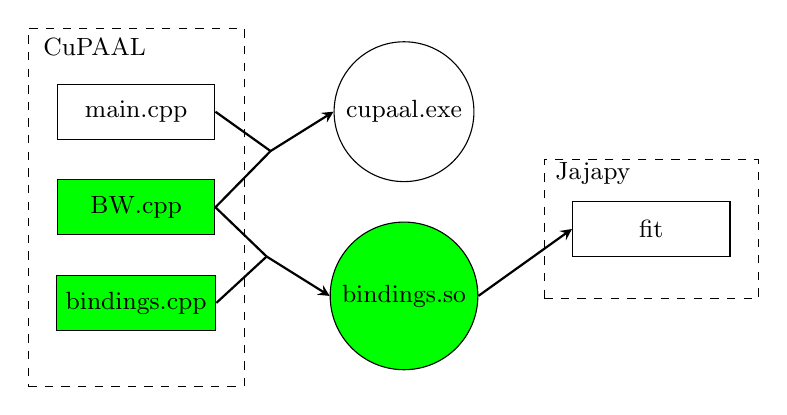
\begin{tikzpicture}[start chain=1 going below,
        start chain=2 going below,
        node distance=.5cm and 1.5cm,
        roundnode/.style={circle, minimum size=7mm, text centered, draw=black, fill=white!30, align=center},
        every node/.style={font=\small}]

    \node [on chain=1, state] (trainingset) {main.cpp} node[below,scale=1, xshift=-15,yshift=30]{CuPAAL};
    \node [on chain=1, state, fill=green] (learning) {BW.cpp};
    \node [on chain=1, state, fill=green] (bind) {bindings.cpp};

    \node [on chain=2, roundnode, right=of trainingset] (cupaal) {cupaal.exe};
    \node [on chain=2, roundnode, fill=green] (bindings) {bindings.so};
    \node [below right=of cupaal, state] (candice) {fit} node[below,scale=1, xshift=165,yshift=-15]{Jajapy};

    \node[draw, dashed, fit={(trainingset) (learning) (bind)},
        inner xsep=10pt, inner ysep=20pt] (box1) {};
    \node[draw, dashed, fit={(candice)},
        inner xsep=10pt, inner ysep=15pt] (box1) {};
    \coordinate (Qf) at ([xshift=-0.8cm, yshift=-0.5cm]cupaal.west);
    \coordinate (Qg) at ([xshift=-0.8cm, yshift=0.5cm]bindings.west);

    \draw[arrow, -] (trainingset.east) --  (Qf);
    \draw[arrow, -] (learning.east) --  (Qf);
    \draw[arrow, -] (bind.east) --  (Qg);
    \draw[arrow, -] (learning.east) --  (Qg);
    \draw[arrow, ->] (Qf) -- (cupaal.west);
    \draw[arrow, ->] (Qg) -- (bindings.west);
    \draw[arrow, ->] (bindings.east) -- (candice.west);
\end{tikzpicture}